\documentclass[11pt,a4paper]{article}
\usepackage[a4paper,top=1.8cm,bottom=1.8cm,left=1.8cm,right=1.8cm]{geometry}
\usepackage{amsmath}
\usepackage[no-math]{fontspec}
\setmainfont{Times New Roman}
\usepackage{newtxmath}
\usepackage{xcolor,colortbl}
\usepackage{array,longtable}
\usepackage{tikz}
\usetikzlibrary{calc,angles,quotes,arrows.meta}
\usepackage{fancyhdr}
\usepackage{titlesec}

\definecolor{hd}{RGB}{31,59,110}
\definecolor{th}{RGB}{226,234,246}
\titleformat{\section}{\Large\bfseries\color{hd}}{}{0pt}{}
\titleformat{\subsection}{\large\bfseries\color{hd}}{}{0pt}{}
\titlespacing*{\section}{0pt}{10pt}{6pt}
\titlespacing*{\subsection}{0pt}{8pt}{4pt}

\pagestyle{fancy}\fancyhf{}\renewcommand{\headrulewidth}{0pt}
\fancyfoot[C]{\small Trang \thepage}

\setlength{\parindent}{0pt}\setlength{\parskip}{3pt}
\renewcommand{\arraystretch}{1.3}
\setlength{\LTpre}{4pt}\setlength{\LTpost}{4pt}

\newcommand{\Cau}[1]{\textbf{Câu #1.}}
\newcommand{\ABCD}[4]{\par\hspace*{1em}%
  \makebox[0.24\linewidth][l]{\textbf{A.} #1}\makebox[0.24\linewidth][l]{\textbf{B.} #2}%
  \makebox[0.24\linewidth][l]{\textbf{C.} #3}\makebox[0.24\linewidth][l]{\textbf{D.} #4}\par}
\newcommand{\hdr}[3]{\rowcolor{th}\textbf{#1} & \textbf{#2} & \textbf{#3}\\ \hline}

\begin{document}

{\LARGE\bfseries\color{hd} Đề Toán THPT mã 901 (2025--2026): lời giải, cấu trúc và đề tương tự\par}
\vspace{4pt}
{\small\color{black!70} Tài liệu do Claude soạn lại bằng lời giải và đề riêng, không sao chép nguyên văn đề gốc. Mọi đáp số đã được kiểm tra lại bằng tính toán (duyệt toàn bộ trường hợp với các câu đếm, tính ký hiệu với giới hạn, toạ độ với hình học). Ảnh đề gốc bị lỗi phông ở ký hiệu tập số trong Câu I.11 và Câu II.7, nên được hiểu lần lượt là $n\in\mathbb N^*$ và $a,b,c\in\mathbb Z$; đáp án không phụ thuộc vào cách hiểu này.\par}

%=====================================================
\section{PHẦN 1. LỜI GIẢI ĐỀ MÃ 901}
\subsection{Phần I. Trắc nghiệm (12 câu)}
\begin{longtable}{|p{0.8cm}|p{13.6cm}|>{\centering\arraybackslash}p{1.2cm}|}
\hline\hdr{Câu}{Hướng giải}{Đáp án}\endhead
1 & Cấp số cộng $u_1=80\,000$, $d=5\,000$, $n=50$: $S_{50}=25\,(2\cdot80\,000+49\cdot5\,000)=10\,125\,000$ đồng. & B\\ \hline
2 & $y=(x+m)^2+m^2+m$ nên đỉnh $I(-m;\,m^2+m)$. $I\in d$: $m^2+m=-m+7\Leftrightarrow m^2+2m-7=0$ ($\Delta'=8>0$). Tổng các giá trị $m$ bằng $-2$. & C\\ \hline
3 & $MF_1\perp MF_2$ nên $OM=c$, suy ra $c^2=\frac95+\frac{16}5=5$, tức $a^2-b^2=5$. Thay $M$ vào $(E)$: $\frac{9}{5a^2}+\frac{16}{5b^2}=1$. Giải ra $a^2=9$, $b^2=4$, vậy $S=a^2+b^2=13$. & D\\ \hline
4 & Tâm $I(3;2)$ là trung điểm $AB$, $R^2=IA^2=4+1=5$: $(x-3)^2+(y-2)^2=5$. & C\\ \hline
5 & Xác suất An, Chi cùng ở bàn $k$ chỗ là $\frac{k}{21}\cdot\frac{k-1}{20}$; cùng bàn mà không kề nhau thì nhân thêm $1-\frac{2}{k-1}$, được $\frac{k(k-3)}{420}$. Tổng: $\frac{18+28+40}{420}=\frac{43}{210}$. & A\\ \hline
6 & Đặt $B(0;0)$, $C(7;0)$, $A=8(\cos40^\circ;\sin40^\circ)$. Dựng $D$ với $AD=3$, $\widehat{BAD}=100^\circ$ (tứ giác lồi) được $CD\approx3{,}516$. Chu vi $\approx21{,}516$ m, chi phí $\approx21{,}516\cdot1{,}8\approx38{,}7$ \$. & A\\ \hline
7 & $f(t)=0\Leftrightarrow t=-1$ hoặc $t=3$. Do $2\cos x\in[-2;2]$ nên chỉ còn $\cos x=-\frac12$. Trên $(0;4\pi)$: $x\in\{\frac{2\pi}3;\frac{4\pi}3;\frac{8\pi}3;\frac{10\pi}3\}$, có 4 nghiệm. & A\\ \hline
8 & Gốc $A$, đặt $\vec{AB}=\vec b$, $\vec{AC}=\vec c$, $\vec{AA'}=\vec a$. $M=\frac{\vec b+\vec c}2$, $P=\vec a+\frac{\vec c}2$ nên $\vec{MP}=\vec a-\frac{\vec b}2$ nằm trong phương của $(ABB'A')$, và $M\notin(ABB'A')$. Vậy $MP\parallel(ABB'A')$. & A\\ \hline
9 & Đặt $\vec{SA}=\vec a$, $\vec{SB}=\vec b$, $\vec{SD}=\vec d$, khi đó $\vec{SC}=\vec b+\vec d-\vec a$. Theo đề: $\vec{SM}=\frac{\vec a}2$, $\vec{SN}=\frac58\vec b$ ($N\in SB$), $\vec{SP}=\frac{\vec b+\vec d-\vec a}2$ ($P$ là trung điểm $SC$). $\vec{SQ}=t\,\vec d$ thuộc $(MNP)$ cho $t=\frac{SQ}{SD}=\frac5{12}$, nên $\frac{QS}{QD}=\frac{5/12}{7/12}=\frac57$. (Cũng có thể dùng $\frac{SA}{SM}+\frac{SC}{SP}=\frac{SB}{SN}+\frac{SD}{SQ}$.) & B\\ \hline
10 & $A(x_1;2\log_2x_1)$, $B(x_2;-\log_2x_2)$. $M$ là trung điểm: $x_1+x_2=12$ và $2\log_2x_1-\log_2x_2=4$, nên $x_1^2=16x_2$. Giải ra $x_1=8$, $x_2=4$: $A(8;6)$, $B(4;-2)$. $(d)\colon 2x-y-10=0$, $d(O,d)=\frac{10}{\sqrt5}=2\sqrt5$. & A\\ \hline
11 & $u_n=5+\sum_{k=1}^{n-1}(3k+2)=\frac{3n^2+n+6}{2}$ (hệ số của $n^2$ là $\frac32$). Giới hạn bằng $\frac{3/2}{2}=\frac34$. & B\\ \hline
12 & $n=30$, $\frac n4=7{,}5$ thuộc nhóm $[80;90)$ (tần số tích luỹ trước đó là 3). $Q_1=80+\frac{7{,}5-3}{6}\cdot10=87{,}5$. & D\\ \hline
\end{longtable}

\subsection{Phần II. Trả lời ngắn (10 câu)}
\begin{longtable}{|p{0.8cm}|p{13.2cm}|>{\centering\arraybackslash}p{1.6cm}|}
\hline\hdr{Câu}{Hướng giải}{Đáp số}\endhead
1 & $|MB-MA|=300\,000\cdot0{,}2\cdot10^{-3}=60$ km nên $M$ thuộc hypebol có $a=30$, $c=50$, $b^2=1600$. Với $y=40$: $\frac{x^2}{900}=2$, $x^2=1800$. $MK=\sqrt{1800+1600}=\sqrt{3400}\approx58{,}31$. & 58,3\\ \hline
2 & Gốc $A$: $G=\frac{2\vec b+\vec d}{3}$. Đường $AG$ cắt đường thẳng $CD$ tại $I$ với $\vec{AI}=2\vec b+\vec d$, nên $\frac{AG}{AI}=\frac13$. $GE\parallel(SCD)\Leftrightarrow GE\parallel SI\Leftrightarrow\frac{AE}{AS}=\frac13$, tức $\frac{SE}{SA}=\frac23$. Vậy $m\cdot n=6$. & 6\\ \hline
3 & $1400=2^3\cdot5^2\cdot7$ nên số có hai chữ số 5, một chữ số 7, ba chữ số còn lại có tích 8: $\{1,1,8\}$, $\{1,2,4\}$, $\{2,2,2\}$. Số hoán vị: $180+360+60=600$. & 600\\ \hline
4 & Miền nghiệm có các đỉnh $(0;0)$, $(7;0)$, $(6;3)$, $(4;5)$, $(0;6)$; $F$ lần lượt bằng $0;\,350;\,210;\,50;\,-180$. Lớn nhất tại $(7;0)$. & 350\\ \hline
5 & Số trên thẻ vàng $\equiv2\pmod3$, thẻ xanh $\equiv3\pmod4$, nên số chung $\equiv11\pmod{12}$ và $\le602$ (thẻ vàng lớn nhất). $11+12k\le602\Rightarrow k=0,\dots,49$: 50 cặp. & 50\\ \hline
6 & $H(0;0)$, $A(0;4)$ (vì $BA=20$), $B(0;24)$, $C(20;32)$. $\tan\widehat{ACB}=\frac{|\vec{CA}\times\vec{CB}|}{\vec{CA}\cdot\vec{CB}}=\frac{400}{624}=\frac{25}{39}$. $a+b=64$. & 64\\ \hline
7 & Mẫu $4x^3-3x+1=(x+1)(2x-1)^2$. Liên tục tại $x=\frac12$ thì tử phải có nghiệm kép $x=\frac12$: $a=b=-3$. Khi đó giới hạn bằng $-2=\frac c2$ nên $c=-4$. $S=abc=-36$. & $-36$\\ \hline
8 & Toạ độ hoá: $S$ cách đều $B,C,D$ nên hình chiếu của $S$ là tâm đường tròn ngoại tiếp $\triangle BCD$; từ $SA=2$ suy ra $\cos\widehat{BAD}=-\frac13$. Mặt phẳng $(P)$ qua $S$ vuông góc $AD$ cắt $AD$ tại $M$ ($AM=\frac1{\sqrt3}$), cắt $BC$ tại trung điểm $N$. Tính được $S_{SMN}=2\sqrt2\approx2{,}83$. & 2,83\\ \hline
9 & Đặt $p=\log_ba$, $q=\log_bc$. Phương trình thành $\frac4{p^2}+\frac{3q-1}{p}+\frac{q(q-1)}2=0$; theo ẩn $\frac1p$ có $\Delta=(q+1)^2$. Do $a,b,c>1$ nên $\frac1p=\frac{1-q}4$. Khi đó $P=\frac4p+1+q=2$. & 2\\ \hline
10 & Có 645 tập con 3 phần tử có tổng 91. Các bộ lập cấp số nhân: $(1,9,81)$, $(7,21,63)$, $(13,26,52)$, $(25,30,36)$, tức 4 bộ. $P=\frac4{645}$ nên $\frac1P=161{,}25$. & 161,25\\ \hline
\end{longtable}
{\small\textit{Ghi chú:} đáp số Câu II.10 có 6 ký tự; nếu phiếu trả lời chỉ có 4 ô như thi tốt nghiệp THPT thì không ghi được. Đây là đặc điểm của đề gốc, không phải sai sót của lời giải.\par}

%=====================================================
\section{PHẦN 2. CẤU TRÚC VÀ MA TRẬN SƠ BỘ CỦA ĐỀ}
Đề gồm hai phần: Phần I có 12 câu trắc nghiệm 4 lựa chọn (3,0 điểm), Phần II có 10 câu trả lời ngắn (7,0 điểm, làm tròn ở bước cuối); thời gian 90 phút, tổng 22 câu. Mức độ dưới đây là đánh giá của Claude, chưa phải của ban ra đề.

\begin{longtable}{|p{1cm}|p{7.2cm}|p{5cm}|p{2.4cm}|}
\hline\rowcolor{th}\textbf{Câu} & \textbf{Nội dung} & \textbf{Chủ đề} & \textbf{Mức}\\ \hline\endhead
I.1 & Tổng tiền khoan giếng & Cấp số cộng (thực tế) & Nhận biết\\ \hline
I.2 & Tham số $m$, đỉnh parabol thuộc đường thẳng & Hàm số bậc hai & Thông hiểu\\ \hline
I.3 & Elip, $MF_1\perp MF_2$ & Phương pháp toạ độ & Vận dụng\\ \hline
I.4 & Đường tròn đường kính $AB$ & Phương pháp toạ độ & Nhận biết\\ \hline
I.5 & Hai bạn ngồi cùng bàn tròn, không kề nhau & Xác suất, tổ hợp & Vận dụng\\ \hline
I.6 & Chi phí rào mảnh đất tứ giác & Hệ thức lượng trong tam giác (thực tế) & Thông hiểu\\ \hline
I.7 & $f(2\cos x)=0$ đọc từ đồ thị & Hàm số, PT lượng giác & Thông hiểu\\ \hline
I.8 & Đường thẳng song song mặt phẳng (lăng trụ) & Quan hệ song song & Nhận biết\\ \hline
I.9 & Tỉ số trên cạnh khi mặt phẳng cắt hình chóp & Quan hệ song song & Vận dụng\\ \hline
I.10 & Khoảng cách tới đường thẳng qua trung điểm & Hàm logarit, toạ độ & Vận dụng\\ \hline
I.11 & Giới hạn của dãy truy hồi & Dãy số, giới hạn & Vận dụng\\ \hline
I.12 & Tứ phân vị mẫu ghép nhóm & Thống kê & Nhận biết\\ \hline
II.1 & Tàu gặp nạn, hiệu thời gian tín hiệu & Hypebol (thực tế) & Vận dụng\\ \hline
II.2 & $GE\parallel(SCD)$, tìm $m\cdot n$ & Quan hệ song song & Vận dụng\\ \hline
II.3 & Số có 6 chữ số, tích các chữ số bằng 1400 & Tổ hợp & Vận dụng\\ \hline
II.4 & Giá trị lớn nhất của $F(x;y)$ trên miền nghiệm & Hệ bất phương trình bậc nhất hai ẩn & Thông hiểu\\ \hline
II.5 & Ghép cặp nhảy theo số trên thẻ & Cấp số cộng, đếm (thực tế) & Vận dụng cao\\ \hline
II.6 & Góc nhìn camera giữa hai toà nhà & Lượng giác (thực tế) & Vận dụng\\ \hline
II.7 & Hàm liên tục tại $x=\frac12$, tìm $abc$ & Giới hạn, hàm số liên tục & Vận dụng cao\\ \hline
II.8 & Chóp đáy hình thoi, diện tích tam giác $SMN$ & Hình học không gian & Vận dụng cao\\ \hline
II.9 & Biểu thức logarit có điều kiện & Mũ, logarit & Vận dụng cao\\ \hline
II.10 & Bộ ba lập cấp số nhân trong tập $\{1,\dots,90\}$ & Xác suất, tổ hợp & Vận dụng cao\\ \hline
\end{longtable}

\textbf{Nhận xét nhanh.}
\begin{itemize}\setlength{\itemsep}{1pt}
\item Thống kê mức độ: Phần I có 4 câu nhận biết, 3 câu thông hiểu, 5 câu vận dụng; Phần II có 1 câu thông hiểu (II.4), 4 câu vận dụng và 5 câu vận dụng cao, tức \textbf{9/10 câu} Phần II ở mức vận dụng trở lên.
\item Kiến thức trộn hai khối: lớp 10 (toạ độ, elip, hypebol, hệ thức lượng, hệ bất phương trình bậc nhất hai ẩn) và lớp 11 (cấp số, giới hạn, quan hệ song song, mũ -- logarit, thống kê ghép nhóm, xác suất).
\item Có 2 câu hình học không gian ở Phần II (II.2, II.8) và \textbf{5 câu có bối cảnh thực tế}: I.1 (khoan giếng), I.6 (rào mảnh đất), II.1 (tàu gặp nạn), II.5 (ghép cặp nhảy), II.6 (camera giữa hai toà nhà).
\item Đề có 5 hình vẽ: I.3, I.6, I.7, II.1, II.6; riêng Câu I.7 bắt buộc đọc thông tin từ đồ thị.
\end{itemize}

%=====================================================
\newpage
\section{PHẦN 3. ĐỀ TƯƠNG TỰ (NỘI DUNG DO CLAUDE SOẠN) VÀ ĐÁP ÁN}
Cùng cấu trúc với đề gốc: 12 câu trắc nghiệm và 10 câu trả lời ngắn, 90 phút; mỗi câu cùng chủ đề và cùng mức độ với câu tương ứng của đề gốc. Số liệu, tình huống và các hình vẽ đều khác đề gốc. Đáp án Phần I phân bố đều: mỗi phương án A, B, C, D đúng 3 lần; đáp số Phần II không quá 4 ký tự.

\subsection{Phần I. Trắc nghiệm}

\Cau{1} Một người gửi tiết kiệm: tháng đầu gửi 2 triệu đồng, mỗi tháng sau gửi nhiều hơn tháng trước 200 nghìn đồng. Sau 24 tháng, tổng số tiền đã gửi là bao nhiêu?
\ABCD{103,2 triệu.}{100,8 triệu.}{110 triệu.}{96 triệu.}

\Cau{2} Cho parabol $(P)\colon y=x^2-2mx+2m^2-m$. Gọi $S$ là tập các giá trị $m$ để đỉnh của $(P)$ nằm trên đường thẳng $y=x+2$. Tổng các phần tử của $S$ là:
\ABCD{$-2$.}{$1$.}{$2$.}{$4$.}

\Cau{3} Trong mặt phẳng $Oxy$, cho elip $(E)\colon\dfrac{x^2}{a^2}+\dfrac{y^2}{b^2}=1$ $(a>b>0)$ có hai tiêu điểm $F_1,F_2$. Biết $(E)$ đi qua điểm $M\left(\dfrac{5\sqrt7}{4};\dfrac94\right)$ và $\widehat{F_1MF_2}=90^\circ$ (hình vẽ). Giá trị của $a^2+b^2$ là:
\begin{center}
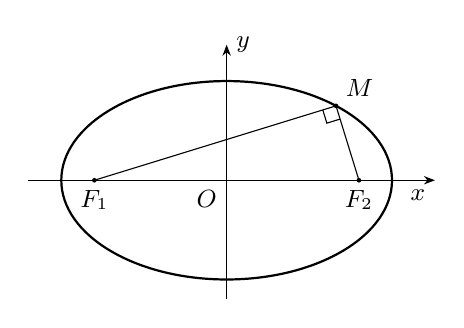
\begin{tikzpicture}[scale=0.42,font=\small]
  \draw[-{Stealth[length=4pt]}] (-6,0) -- (6.3,0) node[below left] {$x$};
  \draw[-{Stealth[length=4pt]}] (0,-3.6) -- (0,4.1) node[right] {$y$};
  \draw[thick] (0,0) ellipse (5 and 3);
  \coordinate (F1) at (-4,0); \coordinate (F2) at (4,0); \coordinate (M) at (3.307,2.25);
  \draw (F1) -- (M) -- (F2);
  \draw pic[draw,angle radius=5pt] {right angle=F1--M--F2};
  \fill (F1) circle (2pt) (F2) circle (2pt) (M) circle (2pt);
  \node[below] at (F1) {$F_1$}; \node[below] at (F2) {$F_2$};
  \node[above right] at (M) {$M$}; \node[below left] at (0,0) {$O$};
\end{tikzpicture}
\end{center}
\vspace{-6pt}
\ABCD{$41$.}{$25$.}{$16$.}{$34$.}

\Cau{4} Đường tròn đi qua ba điểm $O(0;0)$, $A(4;0)$, $B(0;2)$ có bán kính bằng:
\ABCD{$2$.}{$5$.}{$2\sqrt5$.}{$\sqrt5$.}

\Cau{5} Xếp ngẫu nhiên 15 học sinh, trong đó có đúng một bạn tên Lan và đúng một bạn tên Mai, vào hai bàn tròn có 7 chỗ và 8 chỗ, mỗi bạn ngồi một chỗ. Xác suất để Lan và Mai ngồi cùng một bàn nhưng không ngồi cạnh nhau là:
\ABCD{$\dfrac7{15}$.}{$\dfrac{34}{105}$.}{$\dfrac8{35}$.}{$\dfrac13$.}

\noindent\begin{minipage}[t]{0.58\linewidth}
\Cau{6} Bác Hùng có mảnh đất hình tứ giác lồi $ABCD$ với $AB=6$ m, $BC=9$ m, $AD=4$ m, $\widehat{ABC}=50^\circ$, $\widehat{BAD}=110^\circ$ (hình vẽ). Bác rào xung quanh mảnh đất, mỗi mét hàng rào giá $2{,}5$ \$. Số tiền bác phải trả là bao nhiêu (đơn vị: \$, làm tròn đến hàng phần mười)?\par
\hspace*{1em}\textbf{A.} $56{,}3$.\quad \textbf{B.} $55{,}9$.\quad \textbf{C.} $57{,}1$.\quad \textbf{D.} $56{,}8$.
\end{minipage}\hfill
\begin{minipage}[t]{0.38\linewidth}\vspace{0pt}\centering
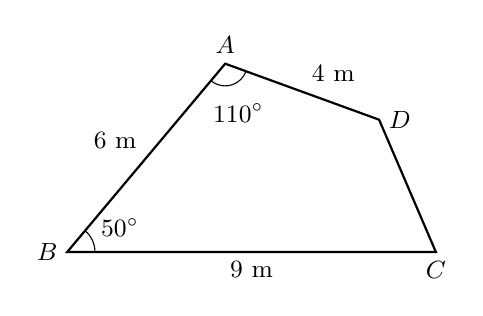
\begin{tikzpicture}[scale=0.52,font=\small]
  \coordinate (B) at (0,0); \coordinate (C) at (9,0);
  \coordinate (A) at (3.857,4.596); \coordinate (D) at (7.615,3.228);
  \draw[thick] (A) -- (B) -- (C) -- (D) -- cycle;
  \node[left] at (B) {$B$}; \node[below] at (C) {$C$};
  \node[above] at (A) {$A$}; \node[right] at (D) {$D$};
  \draw pic["$50^\circ$",draw,angle radius=10pt,angle eccentricity=2.1] {angle=C--B--A};
  \draw pic["$110^\circ$",draw,angle radius=8pt,angle eccentricity=2.3] {angle=B--A--D};
  \node[above left] at ($(A)!0.5!(B)$) {$6$ m};
  \node[below] at ($(B)!0.5!(C)$) {$9$ m};
  \node[above right] at ($(A)!0.5!(D)$) {$4$ m};
\end{tikzpicture}
\end{minipage}

\noindent\begin{minipage}{\linewidth}
\Cau{7} Cho hàm số $f(x)=ax^2+bx+c$ $(a\neq0)$ có đồ thị như hình vẽ. Số nghiệm thuộc khoảng $(0;3\pi)$ của phương trình $f(2\sin x)=0$ là:
\begin{center}
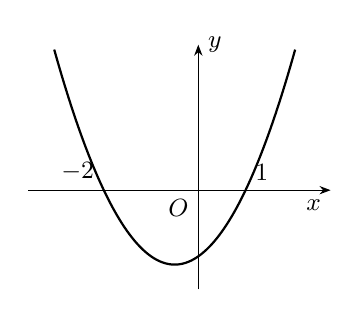
\begin{tikzpicture}[xscale=0.6,yscale=0.42,font=\small]
  \draw[-{Stealth[length=4pt]}] (-3.6,0) -- (2.8,0) node[below left] {$x$};
  \draw[-{Stealth[length=4pt]}] (0,-3) -- (0,4.4) node[right] {$y$};
  \draw[thick,domain=-3.05:2.05,samples=100] plot (\x,{(\x+2)*(\x-1)});
  \node[above left] at (-2,0) {$-2$};
  \node[below left] at (0,0) {$O$};
  \node[above right] at (1,0) {$1$};
\end{tikzpicture}
\end{center}
\vspace{-6pt}
\ABCD{$4$.}{$3$.}{$6$.}{$5$.}
\end{minipage}


\Cau{8} Cho hình hộp $ABCD.A'B'C'D'$. Gọi $M,N$ lần lượt là trung điểm của $AB$ và $A'D'$. Đường thẳng $MN$ song song với mặt phẳng nào dưới đây?
\ABCD{$(ACC'A')$.}{$(ABB'A')$.}{$(BDD'B')$.}{$(CDD'C')$.}

\Cau{9} Cho hình chóp $S.ABCD$ có đáy là hình bình hành. Gọi $M,N$ lần lượt là trung điểm của $SA$, $SC$; $P$ là điểm thuộc cạnh $SB$ sao cho $\dfrac{SP}{SB}=\dfrac23$. Mặt phẳng $(MNP)$ cắt $SD$ tại $Q$. Tỉ số $\dfrac{QS}{QD}$ bằng:
\ABCD{$\dfrac32$.}{$\dfrac23$.}{$\dfrac25$.}{$\dfrac52$.}

\Cau{10} Điểm $A$ thuộc đồ thị hàm số $y=\log_3x$, điểm $B$ thuộc đồ thị hàm số $y=\log_{\frac13}x$ sao cho $M(5;1)$ là trung điểm của $AB$. Độ dài đoạn $AB$ là:
\ABCD{$2\sqrt{17}$.}{$4\sqrt5$.}{$6$.}{$2\sqrt{13}$.}

\Cau{11} Cho dãy số $(u_n)$ xác định bởi $u_1=2$, $u_{n+1}=u_n+4n-1$ với mọi $n\in\mathbb N^*$. Giá trị của $\lim\dfrac{u_n}{4n^2+n-5}$ là:
\ABCD{$\dfrac14$.}{$\dfrac12$.}{$1$.}{$2$.}

\Cau{12} Cho mẫu số liệu ghép nhóm về chiều cao (cm) của một nhóm cây giống:
\begin{center}
\begin{tabular}{|l|c|c|c|c|c|}\hline
Chiều cao & $[60;70)$ & $[70;80)$ & $[80;90)$ & $[90;100)$ & $[100;110)$\\ \hline
Số cây & 4 & 8 & 16 & 8 & 4\\ \hline
\end{tabular}
\end{center}
Tứ phân vị thứ ba $Q_3$ của mẫu số liệu là:
\ABCD{$91{,}25$.}{$93{,}75$.}{$92{,}5$.}{$90{,}5$.}

\subsection{Phần II. Trả lời ngắn (làm tròn ở bước cuối)}

\Cau{1} Hai trạm thu tín hiệu $A$, $B$ đặt trên bờ biển, cách nhau 100 km. Tín hiệu cấp cứu từ tàu $M$ đến trạm $A$ sớm hơn đến trạm $B$ là $0{,}12\cdot10^{-3}$ giây; tín hiệu truyền với vận tốc $300\,000$ km/s. Tàu $M$ cách đường thẳng $AB$ 24 km. Tính khoảng cách từ $M$ đến cảng $K$ là trung điểm của $AB$ (đơn vị: km, làm tròn đến hàng phần mười).
\begin{center}
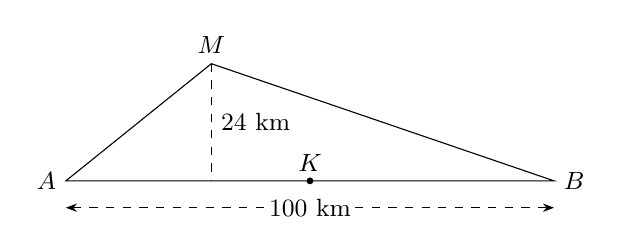
\begin{tikzpicture}[scale=0.62,font=\small]
  \coordinate (A) at (0,0); \coordinate (B) at (10,0); \coordinate (K) at (5,0);
  \coordinate (M) at (2.98,2.4); \coordinate (H) at (2.98,0);
  \draw (A) -- (M) -- (B) -- cycle; \draw[dashed] (M) -- (H);
  \fill (K) circle (2pt);
  \node[left] at (A) {$A$}; \node[right] at (B) {$B$};
  \node[above] at (M) {$M$}; \node[above] at (K) {$K$};
  \node[right] at ($(M)!0.5!(H)$) {24 km};
  \draw[dashed,{Stealth[length=4pt]}-{Stealth[length=4pt]}] (0,-0.55) -- (10,-0.55);
  \node[fill=white,inner sep=1pt] at (5,-0.55) {100 km};
\end{tikzpicture}
\end{center}

\Cau{2} Cho hình chóp $S.ABCD$ có đáy là hình bình hành, $G$ là trọng tâm tam giác $ABC$, $E$ là điểm thuộc cạnh $SA$ thoả mãn $SE=\dfrac mn\,SA$ với $\dfrac mn$ là phân số tối giản. Biết $GE\parallel(SBC)$. Tính $m\cdot n$.

\Cau{3} Có bao nhiêu số tự nhiên có 5 chữ số mà tích các chữ số bằng 360?

\Cau{4} Cho $x,y$ là các số thực không âm thoả mãn $\begin{cases}2x+y\le30\\ x+y\le18\\ x+3y\le36\end{cases}$. Tìm giá trị lớn nhất của biểu thức $F(x;y)=40x-20y$.

\Cau{5} Trong một hội trại, ban tổ chức phát 200 thẻ vàng đánh số lần lượt $4,9,14,19,\dots$ cho 200 bạn nữ và 200 thẻ xanh đánh số lần lượt $2,5,8,11,\dots$ cho 200 bạn nam. Một bạn nam và một bạn nữ thành một cặp chơi trò chơi nếu thẻ của hai bạn mang cùng một số. Có bao nhiêu cặp như vậy?

\noindent\begin{minipage}[t]{0.64\linewidth}
\Cau{6} Hai toà nhà đứng trên mặt đất phẳng, chân của chúng là $H$ và $K$ với $HK=12$ m. Toà nhà 1 cao $BH=16$ m, toà nhà 2 cao $CK=28$ m. Một camera đặt tại đỉnh $C$ của toà nhà 2 để quan sát mặt tường $HB$ của toà nhà 1 (hình vẽ); $A$ và $B$ lần lượt là điểm thấp nhất và cao nhất trên $HB$ mà camera quan sát được, với $\dfrac{BA}{BH}=\dfrac58$. Góc $\widehat{ACB}$ là góc quan sát của camera. Biết $\tan\widehat{ACB}=\dfrac ab$ ($\dfrac ab$ là phân số tối giản). Tính $a+b$.
\end{minipage}\hfill
\begin{minipage}[t]{0.32\linewidth}\vspace{0pt}\centering
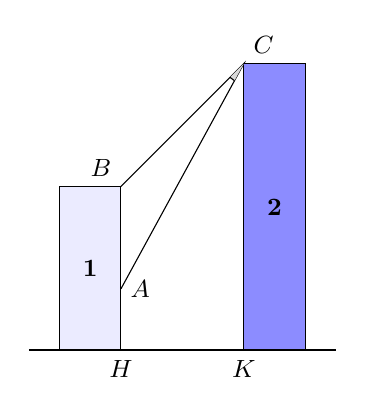
\begin{tikzpicture}[scale=0.13,font=\small]
  \coordinate (H) at (0,0); \coordinate (K) at (12,0);
  \coordinate (B) at (0,16); \coordinate (C) at (12,28); \coordinate (A) at (0,6);
  \fill[blue!8] (-6,0) rectangle (0,16); \draw (-6,0) rectangle (0,16);
  \fill[blue!45] (12,0) rectangle (18,28); \draw (12,0) rectangle (18,28);
  \draw[thick] (-9,0) -- (21,0);
  \draw (B) -- (C) -- (A);
  \draw pic[draw,fill=gray!30,angle radius=7pt] {angle=B--C--A};
  \node at (-3,8) {\textbf{1}}; \node at (15,14) {\textbf{2}};
  \node[above left] at (B) {$B$}; \node[above right] at (C) {$C$};
  \node[right] at (A) {$A$};
  \node[below] at (H) {$H$}; \node[below] at (K) {$K$};
\end{tikzpicture}
\end{minipage}

\Cau{7} Cho hàm số $f(x)=\begin{cases}\dfrac{\sqrt{ax^2+b}-2x-2}{x^3-3x+2} & \text{khi } x\neq1\\[8pt] \dfrac{c}{12} & \text{khi } x=1\end{cases}$ với $a,b,c\in\mathbb Z$. Biết hàm số $f(x)$ liên tục tại $x=1$. Tính $S=abc$.

\Cau{8} Cho hình chóp $S.ABCD$ có đáy $ABCD$ là hình thoi cạnh 4, $SA=3$, $SB=SC=SD=4$. Mặt phẳng $(P)$ đi qua $S$ và vuông góc với $AD$, cắt các đường thẳng $AD$, $BC$ lần lượt tại $M$, $N$. Tính diện tích tam giác $SMN$ (làm tròn đến hàng phần trăm).

\Cau{9} Cho các số thực $a,b,c$ lớn hơn 1 thoả mãn
\[\log^2_{\sqrt[3]{a}}b+\log_ab^6+2\log_bc=\log_b^2c.\]
Tính giá trị của $P=\log_b(bc)-\dfrac{3}{\log_ba}$.

\Cau{10} Cho tập $A=\{1,2,3,\dots,60\}$. Chọn ngẫu nhiên một tập con gồm 3 phần tử của $A$ có tổng các phần tử bằng 63. Gọi $P$ là xác suất để 3 phần tử được chọn lập thành một cấp số nhân. Tính $\dfrac1P$.

\subsection{Đáp án đề tương tự}
\begin{longtable}{|p{1cm}|>{\centering\arraybackslash}p{1.4cm}|p{13.2cm}|}
\hline\hdr{Câu}{Đáp án}{Gợi ý ngắn}\endhead
I.1 & A & $S_{24}=12\,(2\cdot2+23\cdot0{,}2)=103{,}2$ triệu.\\ \hline
I.2 & C & Đỉnh $(m;\,m^2-m)$ thuộc $d$: $m^2-2m-2=0$ ($\Delta'=3>0$), tổng bằng 2.\\ \hline
I.3 & D & $OM=c$: $c^2=\frac{175}{16}+\frac{81}{16}=16$, $a^2-b^2=16$. Thay $M$ vào $(E)$ giải ra $a^2=25$, $b^2=9$; $a^2+b^2=34$.\\ \hline
I.4 & D & $\widehat{AOB}=90^\circ$ nên $AB$ là đường kính, $R=\frac{AB}2=\frac{\sqrt{20}}2=\sqrt5$.\\ \hline
I.5 & B & Cùng bàn $k$ chỗ, không kề nhau: $\frac{k(k-3)}{15\cdot14}$. Tổng $\frac{7\cdot4+8\cdot5}{210}=\frac{68}{210}=\frac{34}{105}$.\\ \hline
I.6 & A & $B(0;0)$, $C(9;0)$, $A=6(\cos50^\circ;\sin50^\circ)$, dựng $D$ (tứ giác lồi) được $CD\approx3{,}513$. Chu vi $\approx22{,}513$ m, chi phí $\approx56{,}3$ \$.\\ \hline
I.7 & D & Đồ thị cắt $Ox$ tại $-2$ và $1$. $2\sin x=1$: $x\in\{\frac\pi6;\frac{5\pi}6;\frac{13\pi}6;\frac{17\pi}6\}$; $2\sin x=-2$: $x=\frac{3\pi}2$. Tổng 5 nghiệm.\\ \hline
I.8 & C & $\vec{MN}=\vec{AA'}+\frac12(\vec{AD}-\vec{AB})=\vec{BB'}+\frac12\vec{BD}$, cùng phương với $(BDD'B')$ và $M\notin(BDD'B')$.\\ \hline
I.9 & B & $\frac{SA}{SM}+\frac{SC}{SN}=\frac{SB}{SP}+\frac{SD}{SQ}$: $4=\frac32+\frac{SD}{SQ}$, $\frac{SQ}{SD}=\frac25$, nên $\frac{QS}{QD}=\frac23$.\\ \hline
I.10 & A & $x_A+x_B=10$, $\log_3x_A-\log_3x_B=2$: $A(9;2)$, $B(1;0)$, $AB=\sqrt{68}=2\sqrt{17}$.\\ \hline
I.11 & B & $u_n=2n^2-3n+3$, giới hạn bằng $\frac24=\frac12$.\\ \hline
I.12 & C & $\frac{3n}4=30$ thuộc nhóm $[90;100)$: $Q_3=90+\frac{30-28}{8}\cdot10=92{,}5$.\\ \hline
II.1 & 31,4 & $2a=36$, $c=50$, $b^2=2176$; $x^2=324\left(1+\frac{576}{2176}\right)$; $MK=\sqrt{x^2+576}\approx31{,}4$.\\ \hline
II.2 & 3 & $AG$ cắt $BC$ tại trung điểm $J$ của $BC$, $\frac{AG}{AJ}=\frac23$; $GE\parallel SJ$ nên $\frac{SE}{SA}=\frac13$, $m\cdot n=3$.\\ \hline
II.3 & 560 & $360=2^3\cdot3^2\cdot5$: đếm các bộ 5 chữ số có tích 360 rồi tính hoán vị (đã kiểm tra bằng duyệt toàn bộ).\\ \hline
II.4 & 600 & Các đỉnh $(0;0)$, $(15;0)$, $(12;6)$, $(9;9)$, $(0;12)$; lớn nhất tại $(15;0)$: $F=600$.\\ \hline
II.5 & 40 & Số chung $\equiv14\pmod{15}$ và $\le599$ (thẻ xanh lớn nhất): $14+15k\le599$, $k=0,\dots,39$: 40 cặp.\\ \hline
II.6 & 22 & $A(0;6)$, $B(0;16)$, $C(12;28)$: $\tan\widehat{ACB}=\frac{120}{408}=\frac5{17}$, $a+b=22$.\\ \hline
II.7 & 128 & Mẫu $=(x-1)^2(x+2)$. Tử có nghiệm kép $x=1$: $\sqrt{a+b}=4$, $\frac{a}{\sqrt{a+b}}=2$, nên $a=b=8$. Giới hạn bằng $\frac{1/2}{3}=\frac16=\frac c{12}$, $c=2$; $abc=128$.\\ \hline
II.8 & 4,68 & $S$ cách đều $B,C,D$ nên hình chiếu của $S$ là tâm đường tròn ngoại tiếp $\triangle BCD$; từ $SA=3$ được $\cos\widehat{BAD}=-\frac7{32}$, chiều cao $2{,}4$. $AM=\frac98$, $N$ là trung điểm $BC$; $S_{SMN}\approx4{,}68$.\\ \hline
II.9 & 3 & $u=\log_ab$, $q=\log_bc$: $9u^2+6u+1=(q-1)^2$, nên $3u+1=|q-1|$; do $u,q>0$ được $q=3u+2$. $P=1+q-3u=3$.\\ \hline
II.10 & 150 & Có 300 tập con có tổng 63; 2 bộ lập cấp số nhân: $(3,12,48)$, $(9,18,36)$. $\frac1P=150$.\\ \hline
\end{longtable}

\end{document}
